\documentclass[a4,10pt,twocolumn]{article}

\usepackage{func}
\usepackage{seminar}

\makeatletter
\author{Hiroshi OCHANOMIZU} % https://ja.wikipedia.org/wiki/%E3%82%A2%E3%83%88%E3%83%A0_%E3%82%B6%E3%83%BB%E3%83%93%E3%82%AE%E3%83%8B%E3%83%B3%E3%82%B0
\title{Research Report}
\date{\today}
\def\@authorInitial{H.O}
\def\@id{01}
\def\@seminar{Robotics research meeting}
\def\@logoimage{hexagon-o.pdf}
%%% Main Document %%%
\begin{document}

\twocolumn[
\renewcommand{\arraystretch}{1.5}
{\centering
\begin{tabular}{p{0.3\textwidth}p{.3\textwidth}p{.3\textwidth}}\hline\hline
\@author &\@authorInitial-\@id&\@date \\ \hline
\multicolumn{3}{P{\textwidth}}{\textbf{\Large\@title}}\\ \hline
\end{tabular}
}
\begin{enumerate}
% Write something you finished.
\item \textbf{Results}
    \begin{enumerate}
        \item First result of research.
        \item Second result of research and more.
    \end{enumerate}
% Write something you will do. 
\item \textbf{Future Work}
	\begin{enumerate}
        	\item First future work
		\item Second future work
    	\end{enumerate}
\end{enumerate}
\begin{tabular}{p{.95\textwidth}}\hline\hline
\\
\end{tabular}
\renewcommand{\arraystretch}{1.0}
]
%\maketitle

%\tiny\scriptsize\footnotesize\small\normalsize\large\Large\LARGE\huge\Huge

\section{Section}
\subsection{Subsection}
\subsubsection{Subsubsection}

\section{Figure and table}\label{result}
\reffig{sample}  is a sample figure recommended to include text over 21pt in 800px width. Graphs and diagrams need to be vector images (pdf or eps). 

Graphs is effective to show  meaning of numbers. Graphs must consist of labels on each axis to clearly meaning of values. Each line of values should have a particular color or a particular line type (solid, doted, etc.).  Lines in the graph need to be with both a particular color  and particular line type. When you draw graphs with MatLab, \textsf{exportfig.m}\footnote{\url{https://github.com/botamochi6277/matlab-exportfig}} may help you.
% If you use [tbp], this figure is on top, the first of this document. I recommend that the first is texts (section).
\begin{figure}[bp]
	\centering
		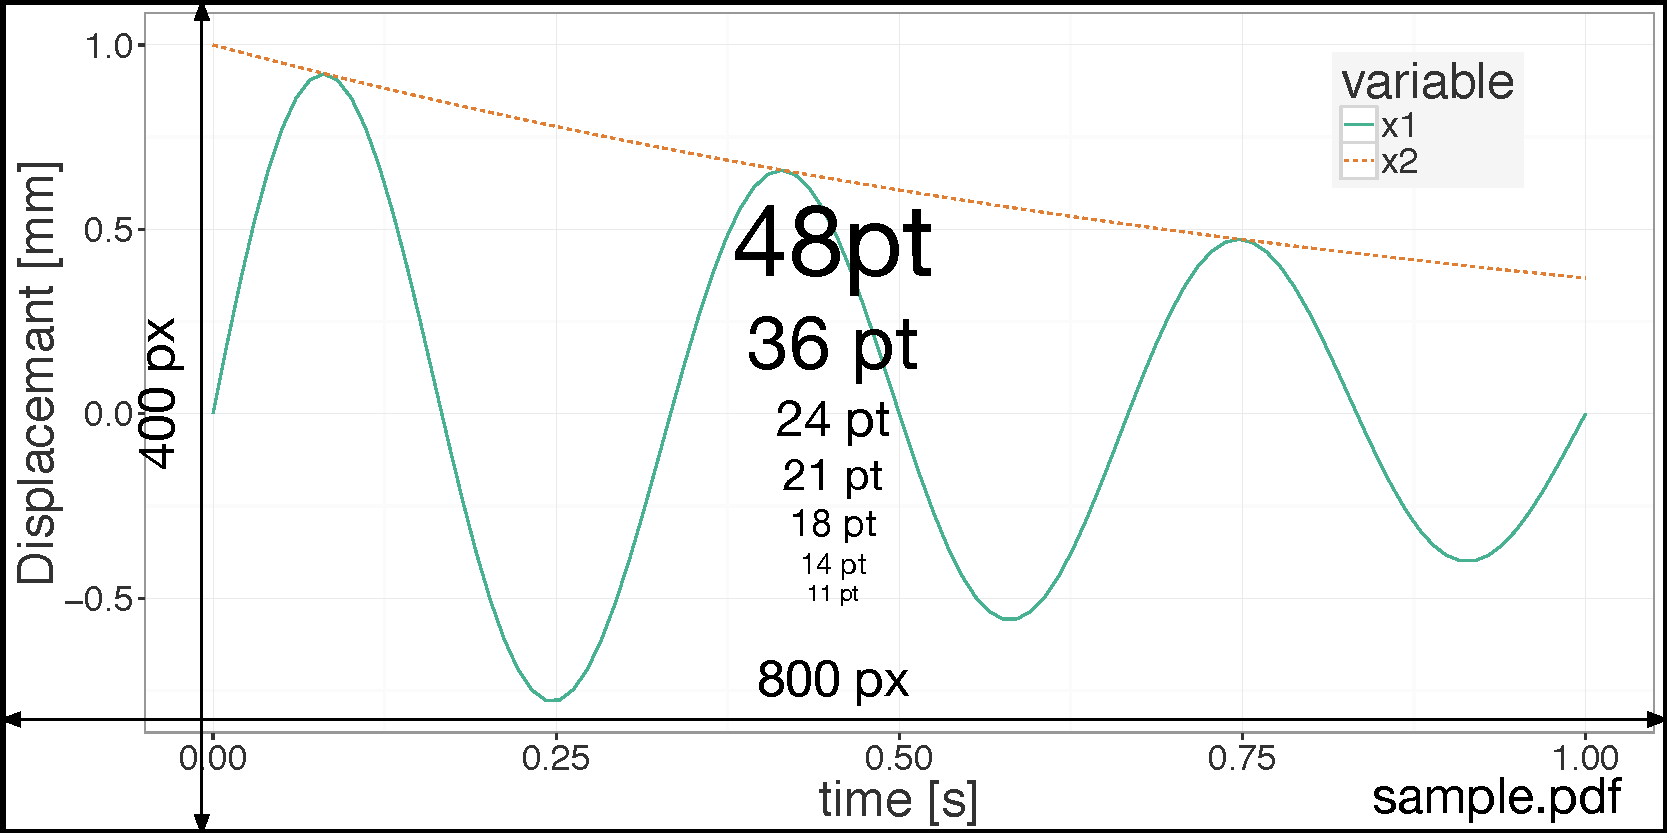
\includegraphics[width=\linewidth]{sample.pdf}
	\caption{Sample figure. Graphs must include labels on axies. Graphs with 2 or more lines needs legends.
	\labfig{sample} 
	}
\end{figure}

\section{Equation}\label{task}
Variables and functions must be written in italics and roman, respectively: $x$ and $\sin x$.
See \refeq{dynamics} and \refeq{oscillation}.

\begin{align}
	m\ddot{x} + c\dot{x} + kx &= F \labeq{dynamics}\\
	x(t) &= e^{\gamma t }(A \cos\omega t + B \sin \omega t) \labeq{oscillation}
\end{align}

\section{Units}
You should use international system of units, SI (\reftab{units}).
%%%%%%%%%%%%%%%%%%%%%%%%%%%%%%%%%%%%%%%%%%%%%%%%%%%%%%%
\begin{table}[tb]
\caption{SI units \labtab{units}}
\centering
\begin{tabular}{ll}\hline\hline
Dimension &	Unit \\ \hline
Length & m, mm, $\mathrm{\mu}$m, nm \\
Mass/weight & kg, g \\
Time & hrs, min, sec, s, ms, $\mathrm{\mu}$s\\ 
Angle & rad, deg \\ \hline
Force & kN, N, mN \\
Pressure/stress & GPa, MPa, kPa, Pa \\ \hline\hline
\end{tabular}
\end{table}%
%%%%%%%%%%%%%%%%%%%%%%%%%%%%%%%%%%%%%%%%%%%%%%%%%%%%%%%


\end{document}
